\documentclass{article}

\title{Architecture document}
\date{8-09-2016}
\author{Robert Kraaijeveld}

\usepackage{graphicx}
\usepackage{fancyhdr}
\usepackage{parskip}

\pagestyle{fancy}
\fancyhead[L]{}


\begin{document}
  \pagenumbering{gobble}
  \maketitle
  \newpage
  \pagenumbering{arabic}
  \tableofcontents

  \newpage
  \section{Introduction}
  In this document, we will give an abstract outline of the structure and architecture of our internship project. 
  This will help us provide a more stable vision for the future of this project and will allow us to divide tasks between ourselves more easily.
  Since we cannot yet predict the exact form that this project will take, the architecture will be presented at quite a high level. We will also
  provide an an abstract view of the algorithms that we intend to use for the procedural generation of avatars with distinct personalities.


  \newpage
  \section{ERD Diagram}
  This very basic ERD Diagram describes the way in which we will separate the Unity-specific code, like providing proxy-properties to Casanova from the abstract Casanova code. In this way, the Casanova code for this project will be completely re-usable within a different framework like XNA or Unreal; only the proxies and the XML writer/reader code will have to be altered or rewritten.

  \begin{figure}[h]
	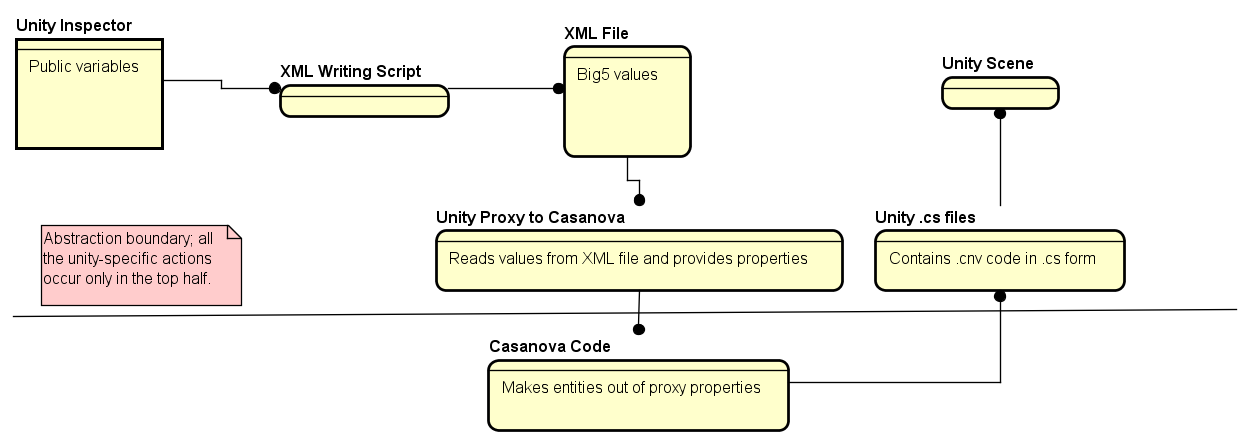
\includegraphics[width=1.4\textwidth]{ER.png}
	\caption{ER-Diagram}
	\label{fig:figure2}
  \end{figure}

  ~\\
  We will most likely provide the big-5 values (or other personality values, more on this later) through an XML file which can be manipulated through the Unity directly inspector. By using an XML file we will be easily able to bring certain personality configurations along on demos and manipulate these configurations from outside of Unity. An important point for us to consider is that the Unity proxies and all other Unity-related pieces of code should not deal with the actual logic of the game; They should only provide an easy interface for Casanova to interact with. By doing this our project will remain relatively independent of Unity, making it easier to use for possible future developers.


  \newpage
  \section{Algorithm structure for a single character}
  In the stages of this project, we will be focusing our attention on having a certain character behave according to his/her personality values and having this character interact with the player accordingly. Characters interacting with other characters is a much more complex subject; we will discuss this in a later chapter. 

  We have identified the most important visible behaviour-characteristics that each avatar should exhibit (almost) regardless of the context of the game in question. There are some exceptions to this rule however, depending on the nature of the game in question. In a relatively static game in which neither player nor npc move around much, like an interrogation-game, movement patterns and walking styles will naturally not be visible. The following list will include examples of each kind of behavior in order to make their distinctions more clear.

  \begin{enumerate}
  	\item Decision-making (Will the character tend to the other NPC who has just fallen over or will I move away?)
  	\item Movement pattern and walking style (Does the NPC move at a steady pace or does he constantly change his walking speed?
  											  Does he walk about confidently or does he slowly wander?) 
  	\item Body Language (What kind of mood does the NPC's body language reflect? Is he standing up proudly or are his shoulders collapsed?)
  	\item Speech (What does the NPC say and with what tone of voice does he say it? What mood does his voice reflect?)
  	\item Facial Expression (Which emotions does the NPC's face reflect? Does his facial expression stay neutral and constant or does it change often and rapidly?)
  \end{enumerate}

  Each of these factors can provide a reasonably visible indication to the player of what kind of personality/emotions the character exhibits. 
  To determine how a certain NPC will display these factors (IE. What the NPC's walking style will be) we will use a personality model. Personality models provide us with a measure of what kind of behavior an NPC who leans to certain sides of a psychological trait would exhibit. 


  \newpage
  \subsection{Change in the behavior of an NPC}
  The behavioral factors of an NPC are changeable and can potentially change for two reasons: Because of the personality of the character itself, or because of certain events that happen to or near the character combined with that characters' personality. Certain personality traits contained in the earlier mentioned personality models, like neuroticism, can cause people to have very variable emotions and extreme emotional reactions to very insignificant events. Within the game, we will likely represent this by having characters with a high neuroticism level change their movement style, body language and facial expression constantly.

  The other way in which we will let our characters behavorial factors change is by subjecting them to certain positive or negative events. Depending on the characters personality, they will respond differently to certain events. An example; NPC 1, who has an egoism value of 100 out of 100 stands next to NPC 2. All of a sudden, NPC 2 lets out a cry of pain and collapses. Because NPC 1 has such a high egoism value, he does not rush to NPC 2's aid: He completely ignores him instead and calmly walks away (An even more cynical reaction might be that NPC 1 starts searching NPC 2 for valuables..).

  If NPC 1 had had a different egoism value, he/she would have reacted differently to this distressing situation. Positive situations will also elicit a certain response depending on the personality values of an NPC. When dance music suddenly starts playing next to a group of NPCs, the extravert ones among them might start to dance, whilst the NPC with very low extraversion scores probably won't dance. 

  Some of the behavorial factors of the NPC's will have to be slightly exagarrated in order for them to be clearly visible to the player and in order for them to be technically viable. Facial expressions in real human beings can be incredible subtle and complex, but emulating exact facial expressions would not only be an incredible technical challenge; it might take extreme player effort in order to actually notice them. Since our focus is still on creating a game, rather than a person simulator, we have prioritized 'playability' over realism.


  \newpage
  \subsection{Our personality models of choice}
   For our first prototype of a single avatar, we will be using the Big 5 personality model. This model has several layers of complexity, but for our very first prototype we will be focusing solely on the top level of the Big 5 model. This personality model containts, as the name implies, 5 principle traits by which to measure personality. They are as follows:

   \begin{itemize}
   	\item Extraversion vs. Introversion
   	\item Egoism vs. Altruism
   	\item Thoroughness vs. Chaoticness \footnote{In the original model, the term 'conscientiousness' is used. Since this term did not seem very descriptive to us, we replaced it with 'Thoroughness'.}
   	\item Emotional Stability vs. Neuroticism 
   	\item Openness to new experiences vs . Stubborness \footnote{Item no. 5 is a little harder to implement as very concrete NPC behavior due to it's relevance lying mostly within the psychological growth and gathering of experiences, therefore we will probably not yet be using much of it in our early prototypes.}
   \end{itemize}

    ~\\
    We have mapped the rest of the factors to the behavioral factors which they will influence:

    ~\\
	\centering
	\label{my-label}
		\begin{tabular}{| p{4cm} | p{4cm} |}
		 \textbf{Behavioral Factor} & \textbf{Big-5 Factor}   \\  \hline
		 Body Language, Speech & Extraversion vs. Intraversion \\  \hline
		 Decision-making & Egoism vs. Altruism    \\  \hline
		 Movement Style & Thoroughness vs. Chaoticness    \\  \hline
 		 Facial Expression & Emotional Stability vs. Neuroticism    
		\end{tabular}
	
	Thusly, the character generation algorithm which we will define will know which personality factor affects the likelihood of a certain behavior factor being exhibited. Next up, we will discuss the actual procedural generation algorithm.

  \newpage
  \subsection{Algorithm structure}
   The algorithm will take as input a list of integers ranging between -100 and 100. Each integer in the list will represent the 'score' for a particular 
   personality factor as defined in the Big five personality model. 

   The score will represent how much the given NPC will exhibit a particular trait; the negative values representing the left side of the two extremes of a particular trait, the positive values representing the right side.

   Given a certain score, the algorithm will take the following (abstract) steps:

   \begin{enum}
   \item Divide the given score by 2. 
   \item If the resulting number is negative, mark this NPC as possessing the left handed trait of the current dicotomy (For instance, Egoism out of 'Egoism vs. Altruism'). Else, mark the NPC as possessing the right handed trait of the current dicotomy.
   \item Whenever the relevant trait of the NPC is triggered\footnote{As mentioned earlier, this can happen due to a positive or negative event or due to the value of a certain trait itself.} use the calculated number to determine how mild or severe the response will be.
   \end{enum}

   It is worth noting that we haven't determined exactly how the mildness or severeness of the NPC response will be turned into actual behavior, but there are a number of options. A simple measure would be to have the calculated number act as a multiplicant for an animation speed variable, or to use it as the duration for a certain animation or state. Slightly more complex measures would be things like having the value of the number decide on a certain animation, walking pattern or action. For instance, the number for egoism could act as the deciding factor regarding wether the earlier mentioned NPC 1 will rob the collapsed NPC 2 or wether he will perform a slightly less egoistic action.

   A potential challenge will be to decide what kind of personality factor is triggered by which kind of external event. There are some no-brainer events of course, like a fellow NPC collapsing on the floor: This event is undoubtedly most relatable to a persons' egoism vs. altruism trait. An alarm that suddenly starts will likely trigger the emotional stability trait of a character, provoking either a mild or severe response from his/her end of the emotional stability vs. neuroticism trait. 

   Other scenarios are much more ambiguous however: The police arriving to arrest an NPC could provoke a lot of different responses: Altruism for the arrestee, Neuroticism at the sight of the police arriving, an extravert response to a particular NPC being arrested, and so on. 
   %DIT UITBREIDDEN


   \newpage
   \section{Differentiating behavioral factor to personality factor bindings}

  %Algorithm steps, inc hoe we de waardes aan persoonlijkheid geven
  %Beschrijving van big5 model en andere modellen; Beginnen met basic big5, dan uitgebreide big5 met facetten, dan hexaco etc.
  %Interactie tussen NPCs
  %'Psychopathietheorie' uitleggen; '' en personality factors zijn niet altijd 1 op 1 het zelfde gekoppeld voor ieder persoon
  %Hoe gaat de demo eruitzien, welke events kiezen we uit

\end{document}